% ------------------------------------------------------------------------------
% Apresentação: Uso de Android Lint para verificação de aderências a guidelines
% Autores:
%     Adorilson Bezerra <adorilson@ppgsc.ufrn.br>
% Licença Creative Commons Atribuição 3.0. 
% Você pode usar e alterar este documento, 
% mas deve obrigatoriamente citar a autoria. 
% ------------------------------------------------------------------------------

\documentclass{beamer}

% ------------------------------------------------------------------------------
\usepackage[latin1]{inputenc}
\usepackage[brazil]{babel}
\usepackage{graphicx}
\usepackage{beamerthemesplit}
\usepackage{ae}
\usepackage{alltt}
\usepackage{pslatex}

\usepackage{xcolor}
% Definindo novas cores
\definecolor{verde}{rgb}{0.25,0.5,0.35}
\definecolor{jpurple}{rgb}{0.5,0,0.35}

% Configurando layout para mostrar codigos Java
\usepackage{listings}
\lstset{
  language=Java,
  basicstyle=\tiny,
  keywordstyle=\color{jpurple}\bfseries,
  stringstyle=\color{red},
  commentstyle=\color{verde},
  morecomment=[s][\color{blue}]{/**}{*/},
  extendedchars=true,
  showspaces=false,
  showstringspaces=false,
  numbers=left,
  numberstyle=\tiny,
  breaklines=true,
  backgroundcolor=\color{cyan!10},
  breakautoindent=true,
  captionpos=b,
  xleftmargin=0pt,
  tabsize=4,
  fontadjust=true,
  basewidth={0.6em,0.45em}
}

% ------------------------------------------------------------------------------

\usecolortheme{beaver}

% ------------------------------------------------------------------------------
\title[Uso de Android Lint para verificação de aderências a guidelines]
{
    Uso de Android Lint para verificação de aderências a guidelines
}
\subtitle{}
\author[Adorilson Bezerra]
{
    Adorilson Bezerra
}
\institute{Universidade Federal do Rio Grande do Norte\\
            Departamento de Informática e Matemática Aplicada}
\date{\today}
%\logo{\includegraphics[scale=0.2]{img/android}}
% ------------------------------------------------------------------------------

\begin{document}

% ------------------------------------------------------------------------------
\frame{\titlepage}
% ------------------------------------------------------------------------------

\section{Introdução}
    \subsection{Motivação}
    \frame
    {
        \frametitle{Motivação}
        \begin{itemize}
            \item Grande variabilidades de dispositivos suportados pela plataforma
            Android
            \begin{itemize}
                \item Tamanho e qualidade de tela, existência ou não de recursos
                como telefone GSM, bluetooth, EDGE, 3G, WiFi, câmera, GPS, bússola, e
                acelerômetro entre outros.
            \end{itemize}
            \item Guideline oficial para tratar essas variabilidades
            \begin{itemize}
                \item Supporting Tablets and Handsets
            \end{itemize}
        \end{itemize}
    }
    \subsection{Problema}
    \frame
    {
        \frametitle{Problema}
        \begin{itemize}
            \item Verificação e aderência a esses padrões é feito de forma manual,
            pelos próprios desenvolvedores
            \item Esses padrões podem ser desconhecidos por eles
            \item Análise estática pode ser utilizada para suprir esse necessidade
        \end{itemize}
    }
    \subsection{Limitações de Trabalhos Atuais}
    \frame
    {
        \frametitle{Limitações de trabalhos atuais}
        \begin{itemize}
            \item Em [Bajwa, 2015] FindBugs e Android Lint são utilizados para mapear
            bugs não-intencionais e vulnerabilidades em aplicações Android a partir
            da analise do código-fonte destas.
            \item Contribuição: uso de analise estática para mapear bugs e vulnerabilidades
            \item continua no slide seguinte...
        \end{itemize}
            
    }
    \frame
    {
        \frametitle{Limitações de trabalhos atuais}
        \begin{itemize}
        \item Pontos positivos:
                \begin{itemize}
                    \item Mapeamento entre bugs e vulnerabilidades, daí a importância
                    evitá-los
                    \item Analise do código-fonte
                    \item Uso de Findbugs e Android Lint
                \end{itemize}
            \item Pontos negativos    
                \begin{itemize}
                    \item Não deixa claro como obteve os projetos do Github (manual ou automático?)
                    \item Não disponibiliza ferramenta e nem detalhes de uso do Findbugs e Lint
                    \item Mostra apenas parte do resultado
                    \item Não estende Lint nem Findbug
                    \item Parte da analise é manual
                    \item O mapeamento é apresentado em nível de categoria de bugs,
                    e não bugs específicos
                \end{itemize}
        \end{itemize}
    }
    \frame
    {
        \frametitle{Limitações de Trabalhos Atuais}
        \begin{itemize}
            \item Em [Khalid et al., 2015] são analisadas 10.000 mil aplicações
            Android gratuitas para download, comparando os resultados encontradas 
            com as críticas feitos pelos usuários
            \begin{itemize}
                \item Utiliza Findbugs, limita-se a usar as validações já pre-definidas
                e analise apenas byte-code
            \end{itemize}
            \item Android Lint é utilizado em [Bugliesi et al., 2013], que propõe um framework
            para checagem de tipos em aplicações Android, com fins de melhorar a
            segurança das aplicações.
            \item Wala\footnote{Disponível em http://wala.sourceforge.net/} também
            é utilizado para analise sintática de aplicações, no entanto, seu suporte
            para análise de código-fonte dos projetos Android é deficitário.
        \end{itemize}
    }
    \frame
    {   
        \frametitle{Limitações de Trabalhos Atuais}
        \begin{itemize}
            \item Em [Saglam, 2014], Android Lint é utilizado na busca por más práticas
            de desenvolvimento, que poderão causar problemas como vazamento e falta
            de memória e travamento de aplicação.
            \begin{itemize}
                \item Valida a abordagem em 100 aplicações open-source, obtidas
                no F-Droid\footnote{https://f-droid.org/}.
                \item Relaciona os resultados obtidos com a avaliação feitas pelos
                usuários da applicação na Google Play
                \item Limitado os aspectos citados, não explora usa de padrões de
                construção
            \end{itemize}
        \end{itemize}
    }
    
    \subsection{Questões de pesquisa}
    \frame
    {
        \frametitle{Questões de pesquisa}
        \begin{itemize}
            \item RQ1: Android Lint pode ser utilizado para guiar os desenvolvedores
                na aplicação de padrões de desenvolvimento?
            \item RQ2: Os desenvolvedores tem aplicados os padrões definidos na
                documentação oficial?
                \begin{itemize}
                    \item RQ2.a: Existem diferenças entre diferentes categorias
                    de aplicações (jogos, educação, negócios etc)?
                \end{itemize}
            \item RQ3: Existem checks predefinidas pelo Android Lint que podem ser
                utilizados para tal fim ? Quais?
            \item RQ4: Novos checks podem ser desenvolvidos?
        \end{itemize}
    }
    
    \subsection{Trabalho proposto}
    \frame
    {
        \frametitle{Trabalho proposto}
        \begin{itemize}
            \item Implementação de novos checks para Android Lint
            \begin{itemize}
            \item Uso de Fragments
                \begin{itemize}
                    \item As activities devem herdar direta ou indiretamente de FragmentActivity
                    \item A activity deve de fato ser composta por fragmentos
                \end{itemize}
            \item Uso de ActionBar
                \begin{itemize}
                    \item As activities devem herdar direta ou indiretamente de ActionBarActivity
                    \item A activity deve usar o tema Theme.AppCompat.Light
                \end{itemize}
            \end{itemize}
            \item{Validação da abordagem através da execução de projetos de código aberto}
        \end{itemize}
    }
    
\section{Android Lint}
    \subsection{Fundamentos do Android Lint}
    \frame
    {
        \frametitle{Fundamentos do Android Lint}
        \begin{itemize}
            \item Android Lint é uma ferramenta de análise de código estática que
            verifica os arquivos fontes de um projeto Android em busca de potenciais
            bugs e melhorias de otimização para corretude, segurana, performance,
            usabilidade, acessibilidade e internacionalização
            \item Pode ser executado integrado com alguma IDE ou na linha de comando
            \item Relatórios em formato HTML e XML
            \item Contem XX checks na versão YY do Android
            \item Permite a escrita de novos checks
        \end{itemize}     
   }
   \subsection{Arquitetura}
   \frame
   {
        \frametitle{Arquitetura}
        \begin{figure}
            \centering
            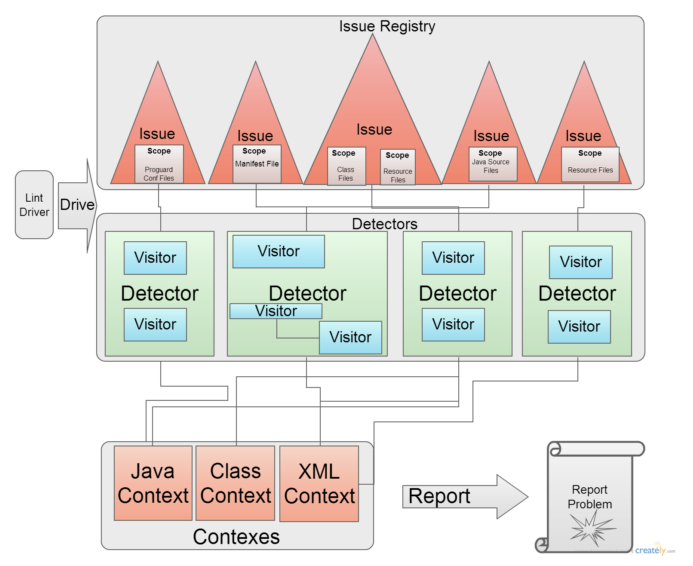
\includegraphics[width=6cm]{img/lint_architecture}
            \caption{Arquitetura do Android Lint (Fonte:[Saglam, 2014])}
            \label{Fonte:[Saglam, 2014]}
        \end{figure}
   }
   \frame
   {
        \frametitle{Arquitetura}
        \begin{itemize}
            \item Detector é uma classe que extende a classe abstrata {\it Detector}
            para procurar por um problema. Um detector pode implementar uma ou mais
            dessas três interfaces: {\it Detector.XmlScanner, Detector.JavaScanner e
            Detector.ClassScanner}
            \item Issues é uma classe de dados com informações, como descrição,
            explicação, categoria e prioridade, sobre o problema procurado por um
            Detector. Scopes define em qual tipo de arquivo de arquivo o problema
            pode surgir. O scope de um issue pode ser arquivos de recursos, código
            fonte Java, arquivos de classes, arquivos de configuração Proguard e
            arquivos manifesto.
         \end{itemize}
   }
   \frame
   {
        \frametitle{Arquitetura}
        \begin{itemize}       
            \item Visitors são classes providas pelo framework que realizam o parser
            nos arquivos e obtem informações deles. O nível mais alto de um visitor
            é a interface AstVisitor que define métodos para percorrer cada nó da 
            arvore sintática abstrata (AST).
            \item Reporting: quando o detector encontra um problema, ele chama o método
            {\it report} do objeto de contexto, que é um objeto de uma subclasse de
            {\it Context}, que pode ser {\it JavaContext, ClassContext e XmlContext}.
            {\it Issue registry: responsável por registrar os novos checks no Lint}
        \end{itemize}
   }
   \frame
   {
        \frametitle{Arquitetura}
        Alguns issues possuem mais de um escopo. Por exemplo, deveria ser analisado
        o arquivo manifesto e o código-fonte Java para encontrar um erro. No entanto,
        a ordem de análise é predefinida, obrigando em alguns casos percorrer os
        arquivos mais de um vez. A ordem definida pelo Lint é:
        \begin{itemize}       
            \item Arquivo manifesto
            \item Arquivos de recursos
            \item Código fonte Java (.java)
            \item Arquivos de classes Java (.class)
            \item Arquivos do Proguard
        \end{itemize}
   }
   \subsection{Exemplificando}
   \frame
   {
        \frametitle{Exemplificando}
        Um detector pode tratar de vários Issue. A seguir veremos um exemplo de
        um detector focando no issue que verifica se as activities herdam de FragmentActivity.
        Serão apresentados os seguintes elementos:
        \begin{itemize}
            \item PatternDetector: classe detector
            \item CHECKFRAGMENTACTIVITY: issue que descreve o problema a ser procurado
            \item PerformanceVisitor: visitor que faz a analise da AST
            \item context.report: chamada ao método report do objeto de context
            \item PatternsIssueRegistry: registra novos issue no Lint
        \end{itemize}
        
   } 

   \frame
   {
    \frametitle{Issue CHECKFRAGMENTACTIVITY}
    \lstinputlisting{Issue.java}
   }
   
   \frame[allowframebreaks]
   {
    \frametitle{Detector PatternsDetector}
    \lstinputlisting{PatternsDetector.java}
   }
   
   \frame[allowframebreaks]
   {
    \frametitle{Visitor PerformanceVisitor e reporting}
    \lstinputlisting{PerformanceVisitor.java}
   }
   
   \frame
   {
    \frametitle{Issue registry PatternsIssueRegistry}
    \lstinputlisting{PatternsIssueRegistry.java}
   }
   
   \frame
   {
    \frametitle{Arquivo MANIFEST.MF (bônus)}
    \lstinputlisting{../src/META-INF/MANIFEST.MF}
   }
   
   \frame
   {
    \frametitle{Diagrama de classes do detector (API)}
    \begin{figure}
            \centering
            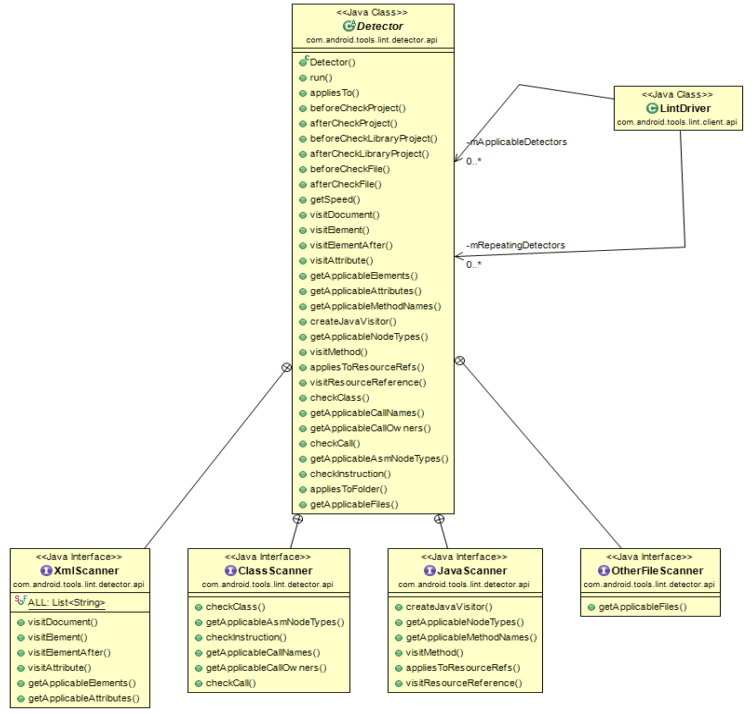
\includegraphics[width=6.5cm]{img/detector_class_diagram}
            \caption{Diagrama de classes do detector (Fonte:[Saglam, 2014])}
            \label{Fonte:[Saglam, 2014]}
        \end{figure}
   }
   
   \frame
   {
    \frametitle{Diagrama de classes do detector implementado}
    \begin{figure}
            \centering
            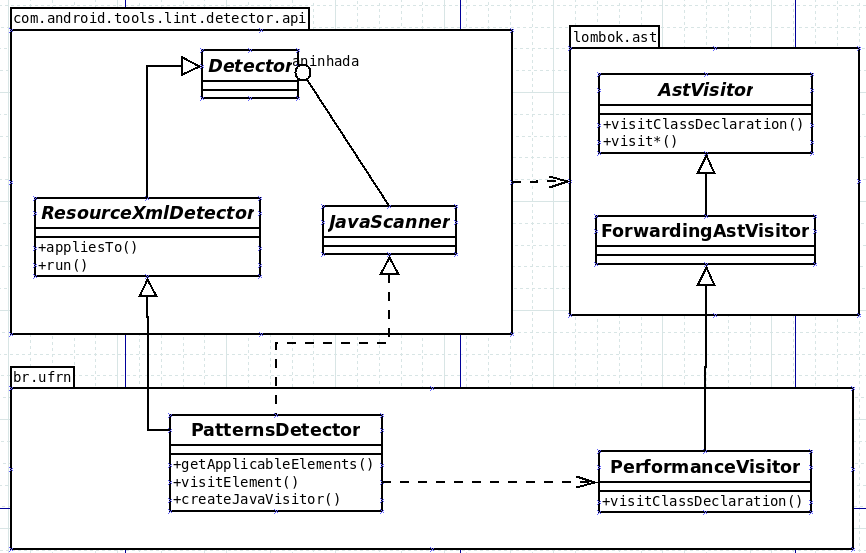
\includegraphics[width=6.5cm]{img/PatternsDetector}
            \caption{Diagrama de classes do detector PatternsDetector}
        \end{figure}
   }
   
    
\section{Resultados parciais}
    \subsection{Resultados parciais}
    \frame
    {
        \frametitle{Resultados Parciais}
        \begin{itemize}
            \item 4 novos checks foram implementados
            \begin{itemize}
                \item 1 deles (checar uso do tema Theme.AppCompat.Light) precisa
                ser refeito para suportar heranças indiretas
            \end{itemize}
            \item{Testados em 3 aplicações: MMUnB, AntennaPod e Google IO Schedule}
                \begin{itemize}
                    \item Apenas no Google IO ocorreu um falso negativo na verificação
                    de heranças devido, provavelmente, estrutura do projeto ou class-loader.
                \end{itemize}
        \end{itemize}
    }

\section{Trabalhos Futuros}
    \subsection{Conclusões e Trabalhos Futuros}
    \frame
    {
        \frametitle{Conclusões e Trabalhos Futuros}
        \begin{itemize}
            \item Finalizar a implementação do check com problema
            \item Executar em larga escala em centenas de aplicações
            \item Colher resultados quantitativos e qualitativos
        \end{itemize}
    }

\section{Bibliografia}
    \subsection{Referencias}
    \frame
    {
        [Bugliesi et al., 2013] Bugliesi, M., Calzavara, S., and Span`o, A. (2013).
        Lintent: Towards security type-checking of android applications. In Beyer,
        D. and Boreale, M., editors, Formal Techniques for Distributed Systems,
        volume 7892 of Lecture Notes in Computer Science, pages 289-304. Springer
        Berlin Heidelberg

        [Khalid et al., 2015] Khalid, H., Nagappan, M., and Hassan, A. (2015).
        Examining the relationship between findbugs warnings and end user ratings:
        A case study on 10,00 android apps. Software, IEEE, PP(99:)1-1

        [Saglam, 2015] Saglam, I. (2014). Measuring and assesment of well known
        bad practices in Android application developments
        
        [Bajwa, 2015] Bajwa, G. and Fazeen, M. and Dantu, R. and Tanpure, S. (2015).
        Unintentional bugs to vulnerability mapping in Android applications. Intelligence
        and Security Informatics (ISI), 2015 IEEE International Conference on, pages 176-178. 
    
    }

\end{document}
